\documentclass[11pt,a4paper]{article}
\usepackage[utf8]{inputenc}
\usepackage{amsmath,amssymb}
\usepackage{algorithm}
\usepackage{algpseudocode}
\usepackage{tikz}
\usetikzlibrary{shapes.geometric, arrows.meta, positioning, calc}
\usepackage[margin=2.5cm]{geometry}
\usepackage{hyperref}

\title{3D Binning Procedure for Diffractive DIS Cross-Section Measurement}
\author{ePIC Collaboration}
\date{}

\begin{document}

\maketitle

\section{Overview}

This document describes the binning optimization procedure for measuring the diffractive reduced cross-section $\sigma_r^{D(3)}(Q^2, \beta, x_\mathbb{P})$ in three dimensions. The methodology follows established HERA practices (ZEUS/H1) adapted for ePIC detector characteristics.

\section{Variable Hierarchy}

The 3D grid is constructed with the following hierarchy:
\begin{enumerate}
    \item \textbf{Master variable:} $Q^2$ -- divided into large slices due to wide dynamic range
    \item \textbf{Secondary variable:} $x_\mathbb{P}$ -- subdivided within each $Q^2$ slice
    \item \textbf{Tertiary variable:} $\beta$ -- distribution measured in each $(Q^2, x_\mathbb{P})$ cell
\end{enumerate}

The global bin index for a 3D cell $(i, j, l)$ corresponding to $(Q^2_i, x_{\mathbb{P},j}, \beta_l)$ is:
\begin{equation}
    k_{\text{global}} = l + j \cdot N_\beta + i \cdot N_\beta \cdot N_{x_\mathbb{P}}
\end{equation}

\section{Pseudocode}

\begin{algorithm}[H]
\caption{3D Binning Optimization Procedure}
\begin{algorithmic}[1]
\Statex \textbf{Phase 1: Resolution Study}
\For{each variable $V \in \{Q^2, x_\mathbb{P}, \beta\}$}
    \State Compute resolution: $\text{Res}_V = \dfrac{V_{\text{rec}} - V_{\text{true}}}{V_{\text{true}}}$
    \State Check correlations (especially $\text{Res}_\beta$ vs $\text{Res}_{x_\mathbb{P}}$)
\EndFor
\Statex
\Statex \textbf{Phase 2: Initial Binning Definition}
\State Define initial bin edges for $Q^2$, $x_\mathbb{P}$, $\beta$
\State Constraint: bin width $\geq 2\text{--}3 \times$ resolution in that region
\Statex
\Statex \textbf{Phase 3: Migration Matrix Construction}
\State Initialize $N_{\text{total}} = N_{Q^2} \times N_{x_\mathbb{P}} \times N_\beta$
\State Create 2D matrix $M[N_{\text{total}}][N_{\text{total}}]$
\For{each MC event}
    \State $k_{\text{gen}} \gets$ GlobalBin($Q^2_{\text{true}}, x_{\mathbb{P},\text{true}}, \beta_{\text{true}}$)
    \State $k_{\text{rec}} \gets$ GlobalBin($Q^2_{\text{rec}}, x_{\mathbb{P},\text{rec}}, \beta_{\text{rec}}$)
    \State $M[k_{\text{gen}}][k_{\text{rec}}] \mathrel{+}= w_{\text{event}}$
\EndFor
\Statex
\Statex \textbf{Phase 4: Purity and Stability Calculation}
\For{each 3D bin $k$}
    \State $\text{Purity}_k = \dfrac{N(\text{rec} \land \text{true in bin } k)}{N(\text{rec in bin } k)}$
    \State $\text{Stability}_k = \dfrac{N(\text{rec} \land \text{true in bin } k)}{N(\text{true in bin } k)}$
\EndFor
\Statex
\Statex \textbf{Phase 5: Bin Merging (if needed)}
\For{each bin $k$}
    \If{$\text{Purity}_k < 0.40$ \textbf{or} $\text{Stability}_k < 0.40$}
        \State Merge bin $k$ with adjacent bin
        \State Recompute migration matrix
        \State Go to Phase 4
    \EndIf
\EndFor
\Statex
\State \Return Optimized bin edges, Migration matrix, Purity/Stability values
\end{algorithmic}
\end{algorithm}

\newpage
\section{Flowchart}

\begin{center}
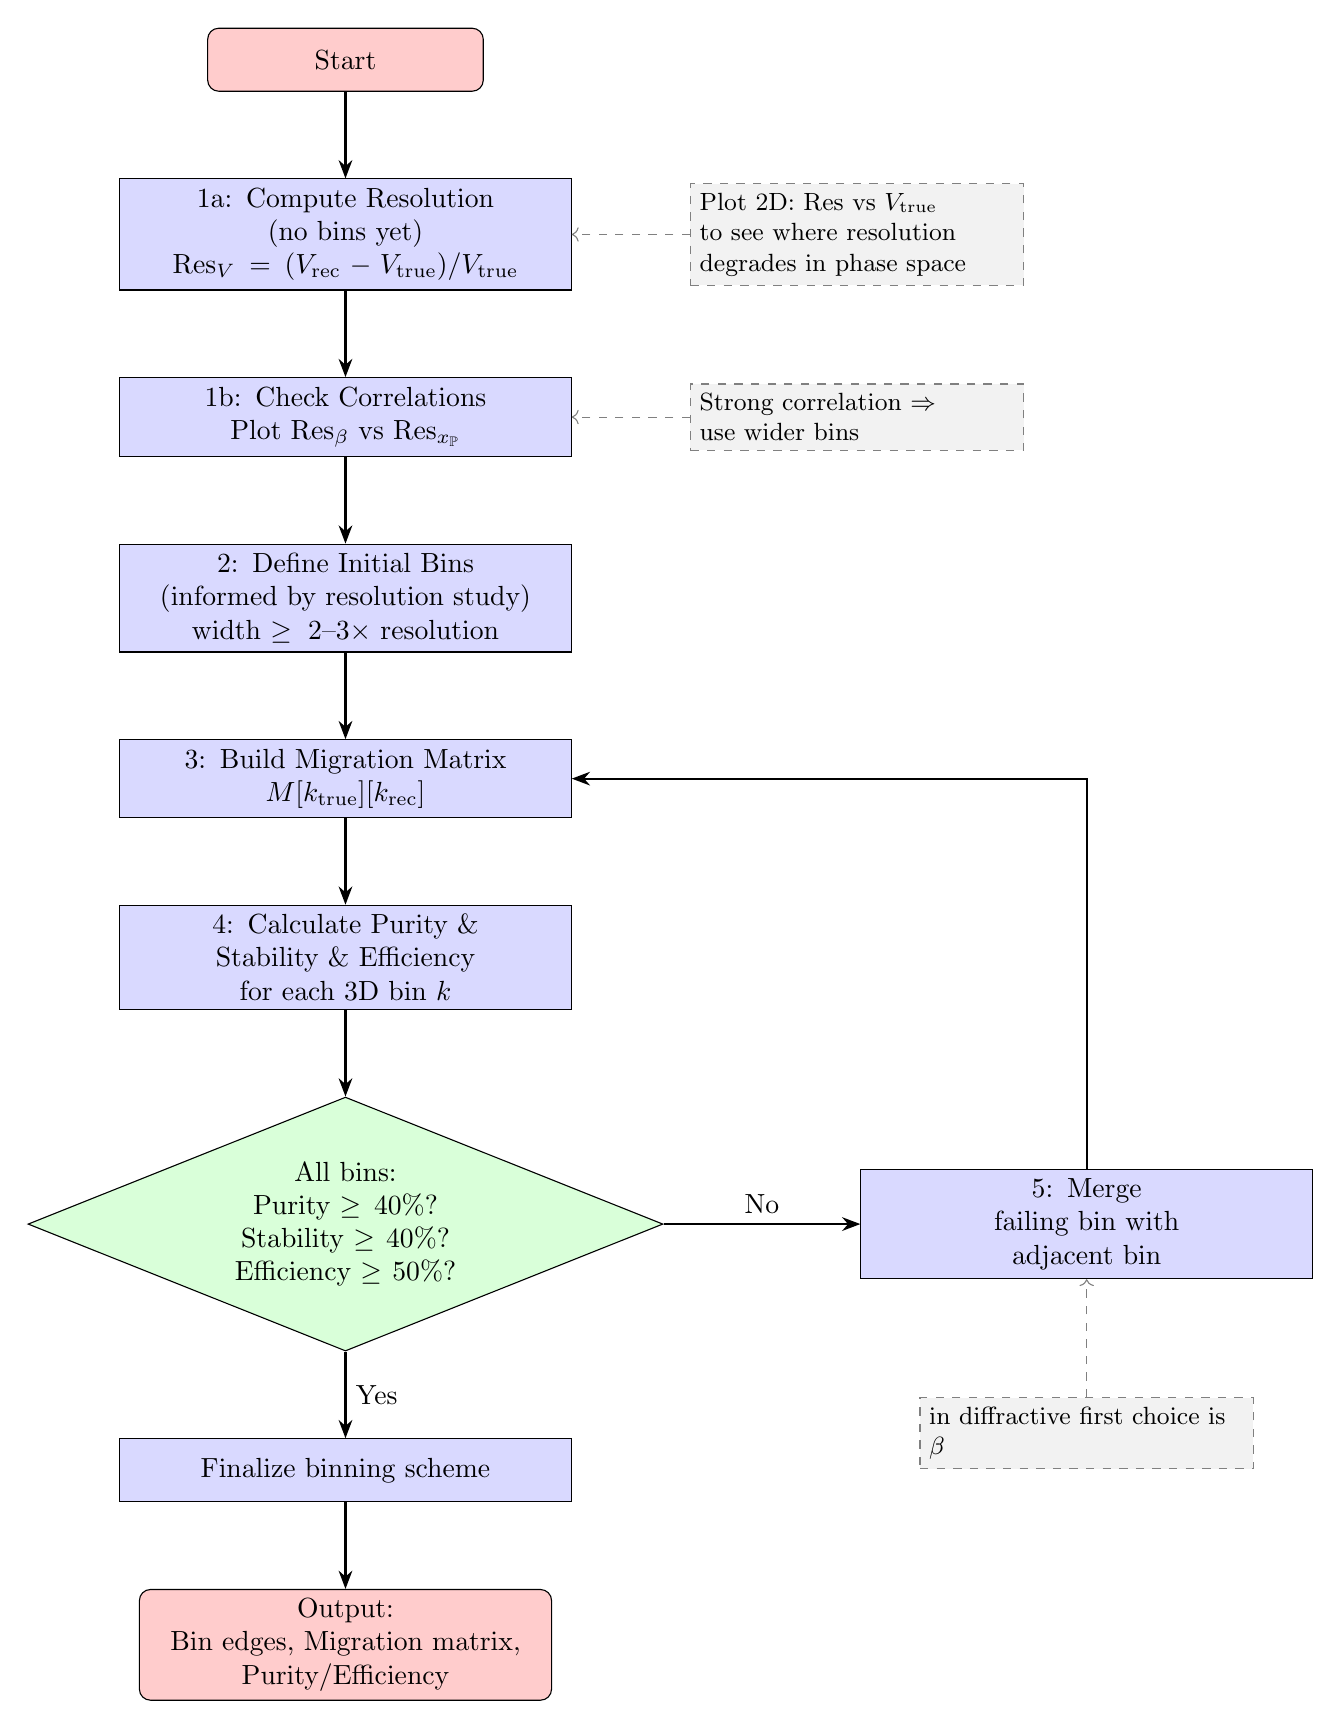
\begin{tikzpicture}[
    node distance=1.1cm,
    startstop/.style={rectangle, rounded corners, minimum width=3.5cm, minimum height=0.8cm, text centered, draw=black, fill=red!20},
    process/.style={rectangle, minimum width=5cm, minimum height=0.8cm, text centered, draw=black, fill=blue!15, text width=5.5cm},
    io/.style={trapezium, trapezium left angle=70, trapezium right angle=110, minimum width=3cm, text centered, draw=black, fill=yellow!20, text width=4cm},
    decision/.style={diamond, minimum width=3cm, minimum height=1cm, text centered, draw=black, fill=green!15, aspect=2.5, text width=2.5cm},
    arrow/.style={thick,->,>=Stealth},
    note/.style={rectangle, draw=gray, dashed, fill=gray!10, text width=4cm, font=\small}
]

% Nodes
\node (start) [startstop] {Start};

\node (res) [process, below=of start] {1a: Compute Resolution\\(no bins yet)\\$\text{Res}_V = (V_\text{rec} - V_\text{true})/V_\text{true}$};

\node (note1) [note, right=1.5cm of res] {Plot 2D: Res vs $V_\text{true}$\\to see where resolution\\degrades in phase space};

\node (corr) [process, below=of res] {1b: Check Correlations\\Plot $\text{Res}_\beta$ vs $\text{Res}_{x_\mathbb{P}}$};

\node (note2) [note, right=1.5cm of corr] {Strong correlation $\Rightarrow$\\use wider bins};

\node (initial) [process, below=of corr] {2: Define Initial Bins\\(informed by resolution study)\\width $\geq 2\text{--}3\times$ resolution};

\node (migrate) [process, below=of initial] {3: Build Migration Matrix\\$M[k_\text{true}][k_\text{rec}]$};

\node (purity) [process, below=of migrate] {4: Calculate Purity \& Stability \& Efficiency\\for each 3D bin $k$};

\node (checkpur) [decision, below=of purity, text width=3.3cm, align=center] {All bins:\\Purity $\geq 40\%$?\\Stability $\geq 40\%$?\\Efficiency $\geq 50\%$?};

\node (merge) [process, right=2.5cm of checkpur] {5: Merge\\failing bin with\\adjacent bin};

\node (note3) [note, below=1.5cm of merge] {in diffractive first choice is $\beta$};

\node (finalize) [process, below=of checkpur] {Finalize binning scheme};

\node (output) [startstop, below=of finalize, text width=5cm, align=center] {Output:\\Bin edges, Migration matrix,\\Purity/Efficiency};

% Arrows
\draw [arrow] (start) -- (res);
\draw [arrow] (res) -- (corr);
\draw [arrow] (corr) -- (initial);
\draw [arrow] (initial) -- (migrate);
\draw [arrow] (migrate) -- (purity);
\draw [arrow] (purity) -- (checkpur);
\draw [arrow] (checkpur) -- node[right] {Yes} (finalize);
\draw [arrow] (checkpur) -- node[above] {No} (merge);
\draw [arrow] (merge) |- (migrate);
\draw [arrow] (finalize) -- (output);

% Dashed info arrows
\draw [dashed, gray, ->] (note1) -- (res);
\draw [dashed, gray, ->] (note2) -- (corr);
\draw [dashed, gray, ->] (note3) -- (merge);

\end{tikzpicture}
\end{center}

\section{Key Formulas}

\subsection{Resolution}
\begin{equation}
    \text{Res}_V = \frac{V_\text{rec} - V_\text{true}}{V_\text{true}}
\end{equation}

\subsection{Global Bin Index}
\begin{equation}
    k = l + j \cdot N_\beta + i \cdot N_\beta \cdot N_{x_\mathbb{P}}
\end{equation}
where $i$, $j$, $l$ are indices for $Q^2$, $x_\mathbb{P}$, $\beta$ bins respectively.

\subsection{Purity and Stability}
\begin{align}
    \text{Purity}_k &= \frac{N^{\text{rec}\land\text{true}}_k}{N^{\text{rec}}_k} \\[0.5em]
    \text{Stability}_k &= \frac{N^{\text{rec}\land\text{true}}_k}{N^{\text{true}}_k}
\end{align}

\subsection{Golden Rules}
\begin{itemize}
    \item Bin width should be $\geq 2$--$3\times$ the resolution in that kinematic region
    \item Migration matrix should be predominantly diagonal
    \item Purity $\geq 40\%$ and Stability $\geq 40\%$ for all bins (ePIC requirement)
    \item Watch for resolution coupling: $\text{Res}_\beta$ depends on $\text{Res}_{x_\mathbb{P}}$
\end{itemize}

\end{document}